\section{Validación}
\label{sec:vali}

En esta sección, se presenta una descripción exhaustiva de los escenarios y pruebas llevadas a cabo para verificar el correcto funcionamiento de las implementaciones realizadas. El propósito de estas pruebas es validar el correcto desempeño de las modificaciones implementadas, tal como se detalla en la sección previa.

Cabe destacar que las pruebas desarrolladas en este capítulo no tienen como objetivo cuantificar el rendimiento del switch BOFUSS por diversas razones. En primer lugar, dicho enfoque no ha sido establecido como objetivo principal del presente TFM (Trabajo de Fin de Máster). En segundo lugar, el switch BOFUSS se encuentra más orientado hacia el prototipado y desarrollo de nuevas funcionalidades que a lograr un rendimiento excepcional en el procesamiento de los paquetes.

En consecuencia, el enfoque de las pruebas se centra en verificar el funcionamiento adecuado de las implementaciones realizadas, sin ahondar en la medición precisa del rendimiento del switch BOFUSS.

\subsection{Comprobación funcional}

% Lets see tomorrow
%\subsection{Comprobación cuantitativa}

% topo eva
\begin{figure}[ht]
    \centering
    \includegraphics[width=0.5\textwidth]{archivos/img/dev/topo_eva.eps}
    \caption{Información ofuscada de la nueva herramienta \texttt{dpctl}}
    \label{fig:topo_eva}
\end{figure}


% topo hellos
\begin{figure}[ht]
    \centering
    \includegraphics[width=0.5\textwidth]{archivos/img/dev/topo_hellos.eps}
    \caption{Información ofuscada de la nueva herramienta \texttt{dpctl}}
    \label{fig:topo_hellos}
\end{figure}


% topo nb - node A
\begin{figure}[ht!]
    \centering
    \includegraphics[width=\textwidth]{archivos/img/dev/topo_hello_nodoA_nb.eps}
    \caption{Información ofuscada de la nueva herramienta \texttt{dpctl}}
    \label{fig:topo_hello_nodoA_nb}
\end{figure}

% topo nb - node B
\begin{figure}[ht!]
    \centering
    \includegraphics[width=\textwidth]{archivos/img/dev/topo_hello_nodoB_nb.eps}
    \caption{Información ofuscada de la nueva herramienta \texttt{dpctl}}
    \label{fig:topo_hello_nodoB_nb}
\end{figure}

% topo nb - node C
\begin{figure}[ht!]
    \centering
    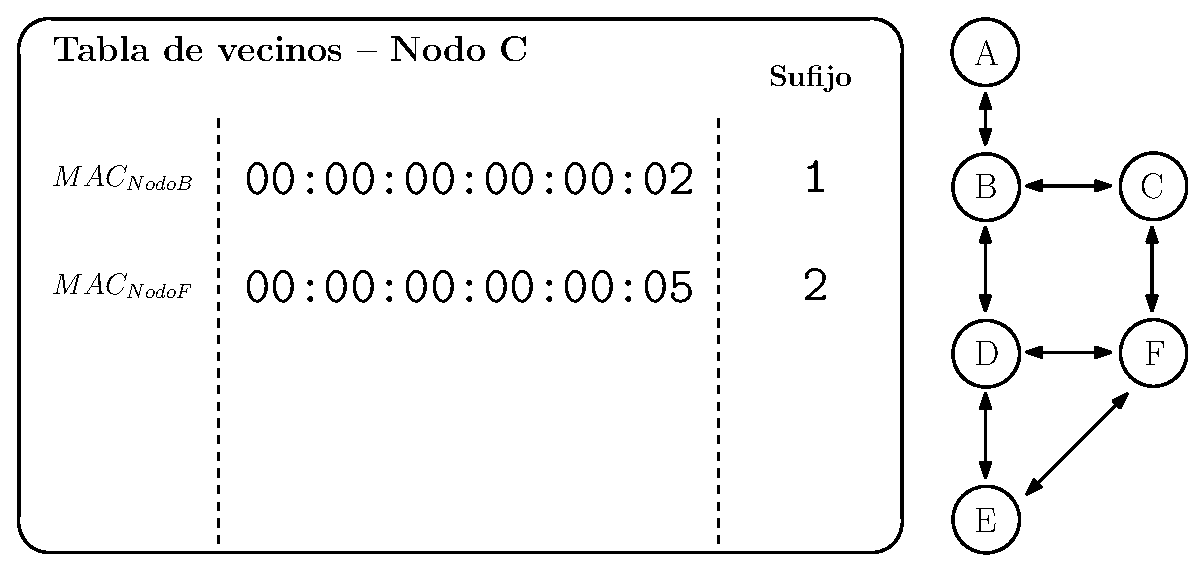
\includegraphics[width=\textwidth]{archivos/img/dev/topo_hello_nodoC_nb.eps}
    \caption{Información ofuscada de la nueva herramienta \texttt{dpctl}}
    \label{fig:topo_hello_nodoC_nb}
\end{figure}


% topo nb - node D
\begin{figure}[ht!]
    \centering
    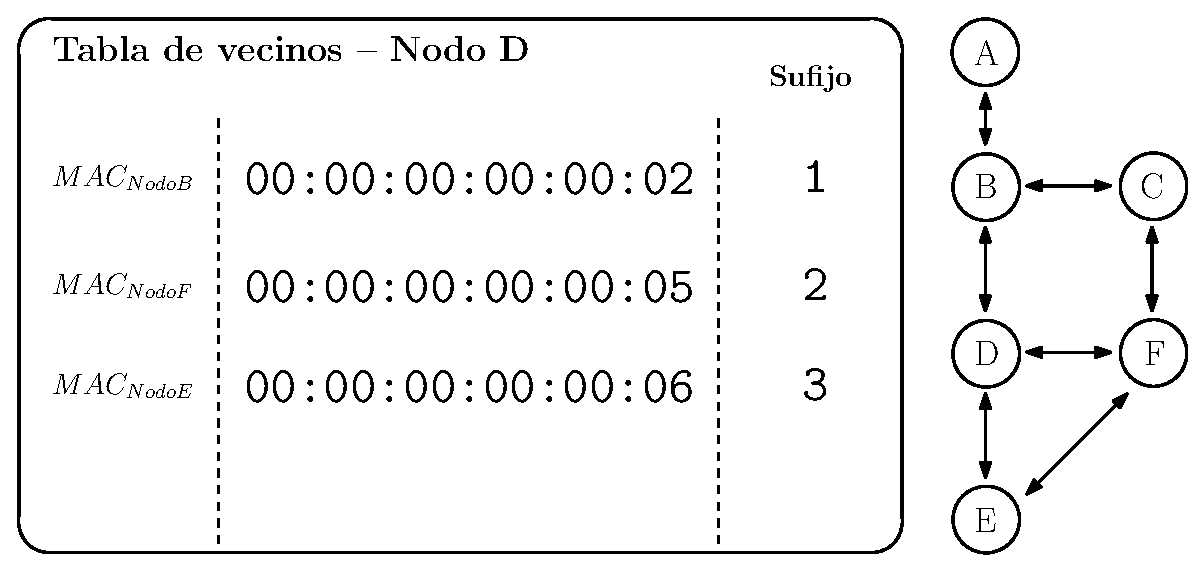
\includegraphics[width=\textwidth]{archivos/img/dev/topo_hello_nodoD_nb.eps}
    \caption{Información ofuscada de la nueva herramienta \texttt{dpctl}}
    \label{fig:topo_hello_nodoD_nb}
\end{figure}


% topo nb - node E
\begin{figure}[ht!]
    \centering
    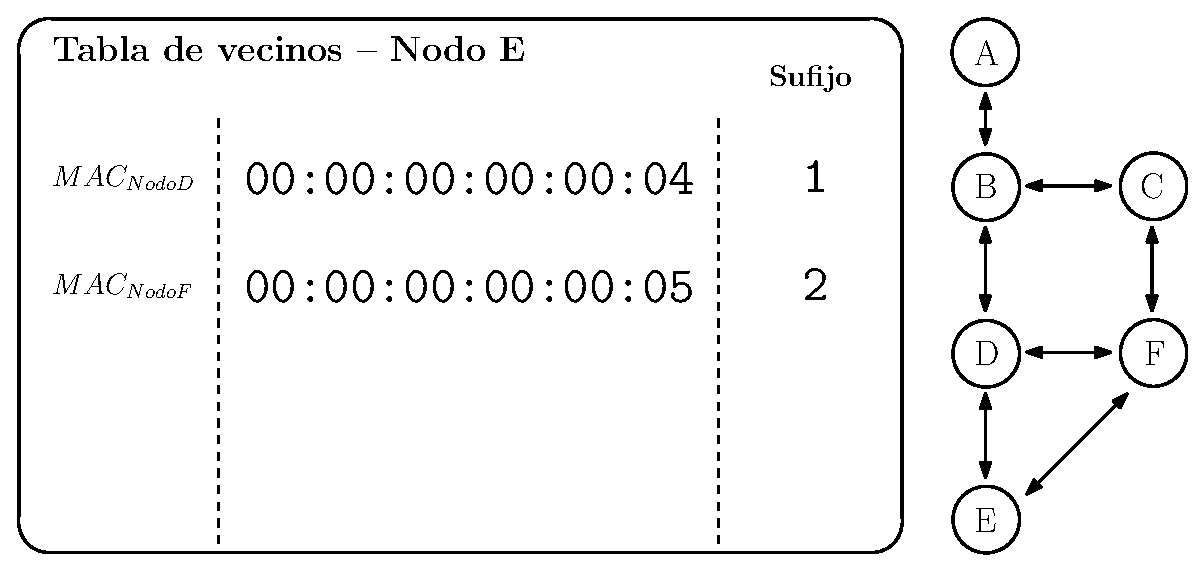
\includegraphics[width=\textwidth]{archivos/img/dev/topo_hello_nodoE_nb.eps}
    \caption{Información ofuscada de la nueva herramienta \texttt{dpctl}}
    \label{fig:topo_hello_nodoE_nb}
\end{figure}


% topo nb - node F
\begin{figure}[ht!]
    \centering
    \includegraphics[width=\textwidth]{archivos/img/dev/topo_hello_nodoF_nb.eps}
    \caption{Información ofuscada de la nueva herramienta \texttt{dpctl}}
    \label{fig:topo_hello_nodoF_nb}
\end{figure}


% topo difu hlmac